\documentclass[10 pt, dvipdfmx]{article}

\usepackage{amsfonts,amsmath,amssymb,amsthm}
\usepackage{bm}
\usepackage{float}
\usepackage{graphicx}
\usepackage{color}
%\usepackage[dvipdfmx]{hyperref}
\usepackage{algorithm}
\usepackage{algorithmic}
%\usepackage{txfonts}
%\usepackage{ascmac, here}
\usepackage{listings}
\usepackage{color}
%\usepackage{url}
\usepackage{comment}

\allowdisplaybreaks[1]

\newtheorem{theorem}{Theorem}
\newtheorem{corollary}{Corollary}
\newtheorem{lemma}{Lemma}
\newtheorem{prop}{Proposition}
%\newtheorem{definition}{Definition}

\theoremstyle{definition}
\newtheorem{definition}{Definition}[section]

%\theoremstyle{remark}
%\newtheorem*{remark}{Remark}

\newcommand{\mysps}{\ensuremath{[\![s^{\otimes}]\!]}_s}
\newcommand{\myspq}{\ensuremath{[\![s^{\otimes}]\!]}_q}
\newcommand{\myspds}{\ensuremath{[\![s^{\otimes \prime}]\!]}_s}
\newcommand{\myspdq}{\ensuremath{[\![s^{\otimes \prime}]\!]}_q}
\newcommand{\argmax}{\mathop{\rm arg~max}\limits}
\newcommand{\argmin}{\mathop{\rm arg~min}\limits}

\begin{document}

\section{System Model}

\begin{definition}
We represent a probabilistic discrete event system (DES) as a labeled Markov decision process (MDP). A DES is a tuple $M$ = $(S, E, \mathcal{E}, P_T, P_E, s_{init}, AP, L)$, where S is a finite set of states; $E$ is a finite set of events; $\mathcal{E} : S \rightarrow E$ is a mapping that maps each state to the set of feasible events at the state; $P_T:S \times S \times E \rightarrow [0,1]$ is a transition probability such that $\sum_{s' \in S} P_T(s'|s,e) = 1$ for any state $s \in S$ and any event $e \in \mathcal{E}(s) $ and $P_T(s'|s,e) = 0$ for any $e \notin \mathcal{E}(s)$; $P_E : E \times S \times 2^E \rightarrow [0,1]$ is the probability that an event occurs under a subset $\pi \in \mathcal{E}(s)$ of events allowed to occur at the state $s \in S$ such that $\Sigma_{e \in \pi} P_E(e|s,\pi) = 1$ and we call the subset the control pattern; for any $(s^{\prime}, s, \pi) \in S \times S \times 2^E$, we define the probability $P : S \times S \times 2^{E} \rightarrow [0,1]$ such that $P(s'|s,\pi) = \sum_{e \in \pi}P_E(e|s,\pi) P_T(s^{\prime}|s,e)$ and $\Sigma_{s^{\prime} \in S} P(s'|s,\pi) = 1$; $s_{init} \in S$ is the initial state; $AP$ is a finite set of atomic propositions; and $L : S \times E \times S \rightarrow 2^{AP}$ is a labeling function that assigns a set of atomic propositions to each transition $(s, e, s') \in S \times E \times S$. We assume that $E$ can be partitioned into the set of controllable events $E_c$ and the set of uncontrollable events $E_{uc}$ such that $E_c \cup E_{uc} = E$ and $E_c \cap E_{uc} = \emptyset$. Note that each event $e$ occurs probabilistically depending on only the current state and the subset of feasible events at the state given by a controller.

In the DES $M$, an infinite path starting from a state $s_0 \in S$ is defined as a sequence $\rho\ =\ s_0e_0s_1 \ldots\ \in S (E S)^{\omega}$ such that $P_T(s_{i+1}|s_i, e_i) > 0$ for any $ i \in \mathbb{N}_0$, where $\mathbb{N}_0$ is the set of natural numbers including zero A finite path is a finite sequence in $S (E S)^*$. In addition, we sometimes represent $\rho$ as $\rho_{init}$ to emphasize that $\rho$ starts from $s_0 = s_{init}$.
For a path $\rho\ =\ s_0e_0s_1 \ldots$, we define the corresponding labeled path $L(\rho)\ =\ L(s_0,e_0,s_1)L(s_1,e_1,s_2) \ldots \in (2^{AP})^{\omega}$.
% We define the set of finite labeled paths as $\mathcal{L}(M) = \{ L(\rho) \in (2^{AP})^{\omega} ; \rho = s_0e_0s_1 \ldots \in S(ES)^{\ast},\ P(s_{i+1}|s_i, e_i) > 0,\ i \in \mathbb{N}_0  \}.
 $InfPath^{M}\ ( \text{resp., }FinPath^{M})$ is defined as the set of infinite (resp., finite) paths starting from $s_0=s_{init}$ in the DES $M$. For each finite path $\rho$, $last(\rho)$ denotes its last state.
\end{definition}

We define the supervisor as a controller for the DES that restricts the behaviors of the DES to satisfy a given specification.

\begin{definition}
For the DES $M$,  a supervisor $SV : FinPath^{M} \rightarrow 2^E$ is defined as a mapping that maps each finite path to a set of enabled events at the finite path and we call the set a control pattern. Note that the relation $E_{uc} \subset SV(\rho) \subset E$ holds for any $\rho \in FinPath^M$.
\end{definition}


\begin{definition}
  A state $\bar{x}$ in the state set $\bar{X}$ of an augmented tLDBA $\bar{B}_{\varphi} = (\bar{X}, \bar{x}_{init},\bar{\Sigma},\bar{\delta},\bar{\mathcal{F}})$ is a sink state if no accepting transition is defined for all states reachable from $\bar{x}$. We denote the set of sink states as $Sink Set$.
\end{definition}

\begin{definition}
  Given an augmented tLDBA $\bar{B}_{\varphi} = (\bar{X}, \bar{x}_{init},\bar{\Sigma},\bar{\delta},\bar{\mathcal{F}})$ and a DES $M$, a tuple $M \otimes \bar{B}_{\varphi} = M^{\otimes} = (S^{\otimes}, E^{\otimes}, {\mathcal E}^{\otimes}, s_{init}^{\otimes}, P^{\otimes}_T, P^{\otimes}_E, \delta^{\otimes}, {\mathcal F}^{\otimes})$ is a product DES, where
  $S^{\otimes} = S \times \bar{X}$ is the finite set of states and we represent $s$ and $\bar{x}$ corresponding with $s^{\otimes} = (s,\bar{x}) \in S^{\otimes}$ as $\mysps$ and $\myspq$, respectively, $E^{\otimes}=E$ is the finite set of events, ${\mathcal E}^{\otimes} : S^{\otimes} \rightarrow 2^{E^{\otimes}}$ is the mapping defined as ${\mathcal E}^{\otimes}((s,\bar{x})) = {\mathcal E}(s)$, $s_{init}^{\otimes} = (s_{init},\bar{x}_{init})$ is the initial states, $P^{\otimes}_T : S^{\otimes} \times S^{\otimes} \times E^{\otimes} \rightarrow [0,1]$ is the transition probability defined as
  \begin{align}
    P^{\otimes}_T(s^{\otimes \prime} | s^{\otimes}, e) =
    \left\{
    \begin{aligned}
      &P_T(s^{\prime} | s, e) &   &\text{if}\  (\bar{x}, L((s,e,s^{\prime})), \bar{x}^{\prime}) \in \bar{\delta},\\
      &0 &   &\text{otherwise} ,
    \end{aligned}
    \right. \nonumber
  \end{align}
  $P^{\otimes}_E : E^{\otimes} \times S^{\otimes} \times 2^{E^{\otimes}} \rightarrow [0,1]$ is the probability of the occurrence of the event defined as $P^{\otimes}_E(e | s^{\otimes}, \pi) = P_E(e | s, \pi)$, $\delta^{\otimes} = \{ (s^{\otimes}, e, s^{\otimes \prime}) \in S^{\otimes} \times E^{\otimes} \times S^{\otimes} ; P^{\otimes}_T(s^{\otimes \prime} | s^{\otimes}, e) > 0 \}$ is the set of transitions, and ${\mathcal F}^{\otimes} = \{ \bar{F}^{\otimes}_1, \ldots ,\bar{F}^{\otimes}_n \}$ is the acceptance condition, where $\bar{F}^{\otimes}_i = \{ ((s,\bar{x}), e, (s^{\prime}, \bar{x}^{\prime})) \in \delta^{\otimes}\ ;\ (\bar{x}, L(s,e,s^{\prime}), \bar{x}^{\prime}) \in \bar{F}_i \}$ for each $ i \in \{ 1, \ldots ,n \}$.
\end{definition}

In the following, the supervisor for the product DES $M^{\otimes}$ we consider is {\it state-based}, namely for any $\rho \in FinPath^{M^{\otimes}}$, $SV(\rho) = SV(last(\rho))$.

\section{Objective function for Control patterns}
From the view point of reinforcement learning, the DES can be interpreted as the environment controlled by the supervisor and the supervisor can be interpreted as the agent. We introduce the two following assumptions.

\begin{enumerate}
  \item The relative frequency of occurrence of each event does not depend on the control pattern.
  \item We define a reward function $\mathcal{R} : S \times 2^E \times E \times S \rightarrow \mathbb{R}$ and the reward $\mathcal{R}$ can be decomposed into $\mathcal{R}_1$ and $\mathcal{R}_2$. The first reward $\mathcal{R}_1 : S \times 2^E \rightarrow \mathbb{R}$ is a reward that is determined by the control pattern selected by the supervisor, which depends on only the control pattern and the current state. The second reward $\mathcal{R}_2 : S \times E \times S \rightarrow \mathbb{R}$ is a reward that is determined by the occurrence of an event and the corresponding state transition. For any $(s,\pi,e,s^{\prime}) \in S \times 2^E \times E \times S$, we then have
  \begin{align}
    \mathcal{R}(s,\pi,e,s^{\prime}) = \mathcal{R}_1(s,\pi) + \mathcal{R}_2(s,e,s^{\prime}).
  \end{align}
\end{enumerate}
Under the above assumptions, we have the following {\it Bellman optimality equation}.

\begin{align}
  Q^{\ast}(s,\pi) = & \sum_{s^{\prime} \in S} P(s^{\prime}|s,\pi)\nonumber \\
  & \left \{ \mathcal{R}(s,\pi,e,s^{\prime}) + \gamma \max_{\pi^{\prime} \in 2^{\mathcal{E}(s^{\prime})}} Q^{\ast}(s^{\prime},\pi^{\prime}) \right \} \nonumber \\
  = & \sum_{s^{\prime} \in S} \sum_{e \in \pi} P_Ee|s,\pi) P_T(s^{\prime}|s,e) \left \{ \mathcal{R}_1(s,\pi) + \mathcal{R}_2(s,e,s^{\prime}) + \gamma \max_{\pi^{\prime} \in 2^{\mathcal{E}(s^{\prime})}} Q^{\ast}(s^{\prime},\pi^{\prime}) \right \} \nonumber \\
  = & \mathcal{R}_1(s,\pi) + \sum_{e \in \pi} P_E(e|s,\pi) \sum_{s^{\prime \in S}} P_T(s^{\prime}|s,e) \left \{ \mathcal{R}_2(s^{\prime}|s,e) + \gamma \max_{\pi^{\prime} \in 2^{\mathcal{E}(s^{\prime})}} Q^{\ast}(s^{\prime}, \pi^{\prime}) \right \},
\end{align}
where $\gamma \in [0,1)$.

We introduce the following function. $T^{\ast} : S \times E \rightarrow \mathbb{R}$ such that
\begin{align}
  T^{\ast}(s,e) = \sum_{s^{\prime \in S}} P_T(s^{\prime}|s,e) \left \{ \mathcal{R}_2(s^{\prime}|s,e) + \gamma \max_{\pi^{\prime} \in 2^{\mathcal{E}(s^{\prime})}} Q^{\ast}(s^{\prime}, \pi^{\prime}) \right \}.
\end{align}
We then have
\begin{align}
  Q^{\ast}(s,\pi) = \mathcal{R}_1(s,\pi) + \sum_{e \in \pi}P_E(e|s,\pi) T^{\ast}(s,e).
\end{align}
\begin{definition}
We define an optimal supervisor $SV^{\ast}$ as follows. For any state $s \in S$,
\begin{align}
  SV^{\ast}(s) = \pi^{\ast} \in \argmax_{\pi \in \mathcal{E}(s)} Q^{\ast}(s,\pi).
\end{align}
\end{definition}

\begin{definition}
  The two reward functions $\mathcal{R}_1 : S^{\otimes} \times 2^{E^{\otimes}} \rightarrow \mathbb{R}$ and $\mathcal{R}_2 : S^{\otimes} \times E^{\otimes} \times S^{\otimes} \rightarrow \mathbb{R}$ are defined as follows.
  \begin{align}
    \mathcal{R}_1 (s^{\otimes}, \pi) =
    \left\{
    \begin{aligned}
      & r_{n}|\pi| & &\text{if} \ \myspq \notin SinkSet , \\
      & 0 & &\text{otherwise},
    \end{aligned}
    \right.
  \end{align}
  where $|E|$ means the number of elements in the set $E$ and $r_{n}$ is a positive value.
  \begin{align}
    \mathcal{R}_2(s^{\otimes}, e, s^{\otimes \prime}) =
    \left\{
    \begin{aligned}
      &r_p & & \text{if}\ \exists j \in \! \{ 1, \ldots ,n \},\ (s^{\otimes}, e, s^{\otimes \prime}) \in \bar{F}^{\otimes}_j \!,\\
      &r_{sink} & & \text{if}\ \myspdq \in SinkSet,\\
      &0 & & \text{otherwise},
    \end{aligned}
    \right.
  \end{align}
  where $r_p$ and $r_{sink}$ are the positive and negative value, respectively.
  \label{reward_def}
\end{definition}

\section{Learning Algorithm}
We make the supervisor learn how to give the control patterns to satisfy an LTL specification while keeping costs associated with prohibited events low. We use Q-learning to estimate the function $T^{\ast}$. We then use Bayesian inference to robustly estimate the probability $P_E$. For the inference, we model $P_E$ as Categorical distribution as $p^k_{s,\pi,e}$, where $p^k_{s,\pi,e}$ represents the estimated probability of $P_E(e|s,\pi)$ at the time step $k$ and the prior distribution $\phi^k_{s,\pi}$ for the distribution of the parameter of $p^k_{s,\pi,e}$ is defined as Dirichlet.
%Let $\mathcal{P}_{s,\pi}$ be the collection of the estimated probabilities of $P_E(e|s,\pi)$ with respect to all $e \in \pi$.

In the following, we distinguish events by numbering them as $\{ e^1, \ldots, e^{|E|} \}$ . To reflect the events prohibition by the supervisor on the estimated probability of the occurrence of allowed events, we introduce the function $RestProb : (0,1)^{|E|} \times 2^E \rightarrow [0,1]^{|E|}$ defined as

\begin{align}
  RestProb(\phi^k_{s,\pi},\pi)_i =
  \left\{
  \begin{aligned}
    & \frac{\phi^{k,i}_{s,\pi}}{\sum_{e^j \in \pi} \phi^j_{s,\pi}} \  &\text{if}\ e^i \in \pi,\\
    &0   \ &\text{otherwise},
  \end{aligned}
  \right.
\end{align}
where $\phi^{k,i}_{s,\pi}$ is the $i$-th element of $\phi^k_{s,\pi}$ and $RestProb(\phi^k_{s,\pi},\pi)_i$ is the $i$-th element of $RestProb(\phi^k_{s,\pi},\pi)$.

We denote the probability vector of a event occurrence at the time step $k$ as $p^k_{s,\pi} = (p^k_{s,\pi,e^1}, \ldots, p^k_{s,\pi,e^{|E|}})$, where $s \in S$ and $\pi \in \mathcal{E}(s)$ is the state and the control pattern at the time step $k$. Let $n^k_{s,\pi,e}$ be the number of the occurrence of the event $e \in E$ up to the time step $k$ at the state $s \in S$ under the control pattern $\pi \in \mathcal{E}(s)$, let $n^k_{s,\pi} = (n^k_{s,\pi,e_1}, \ldots, n^k_{s,\pi,e_{|E|}})$, and let $\bar{p}^k_{s,\pi}$ denote the expected value of $p^k_{s,\pi}$. We sample the parameter $\phi^k_{s,\pi}$ of the posterior distribution of the event occurrence from the Dirichlet distribution $Dir(\cdot|n^k_{s,\pi})$. Then, we obtain the estimated probability vector $p^k_{s,\pi}$ of an event occurrence by $RestProb$ from the sampled parameter $\phi^k_{s,\pi}$ and the control pattern $\pi$. We repeat the procedure until $||p^k_{s,\pi} - \bar{p}^k_{s,\pi}||_1 < \xi^k_{s,\pi}$ holds.

The overall procedure of the inference is shown in Algorithm \ref{bayes}.

\begin{algorithm}[H]
 \caption{$P_E$ inference.}
 \begin{algorithmic}[1]
 \renewcommand{\algorithmicrequire}{\textbf{Input:}}
 \renewcommand{\algorithmicensure}{\textbf{Output:}}
 \REQUIRE the event occurrence count $n^k_{s,\pi}$, a threshold $\xi^k_{s,\pi}$ for $p^k_{s,\pi}$
 \ENSURE  the posterior distribution $p^k_{s,\pi}$
  \REPEAT
  \STATE $\phi^k_{s,\pi} \sim Dir(\cdot|n^k_{s,\pi})$
  \STATE $p^k_{s,\pi} = RestProb(\phi^k_{s,\pi},\pi)$
  \UNTIL $||p^k_{s,\pi} - \bar{p}^k_{s,\pi}||_1 < \xi^k_{s,\pi}$
 \end{algorithmic}
 \label{bayes}
 \end{algorithm}

Under the estimation of $P_E$, we use TD-learning to estimate $Q^{\ast}$ with the TD-error defined as $\mathcal{R}_1(s^{\otimes},\pi) + \sum_{e \in \pi} p_{\mysps,\pi,e} T(s^{\otimes},e) - Q(s^{\otimes},\pi)$.

We show the overall procedure of the learning algorithm in Algorithm \ref{alg1}.

\begin{algorithm}[H]
 \caption{RL-based synthesis of a supervisor satisfying the given LTL specification.}
 \begin{algorithmic}[1]
 \renewcommand{\algorithmicrequire}{\textbf{Input:}}
 \renewcommand{\algorithmicensure}{\textbf{Output:}}
 \REQUIRE LTL formula $\varphi$, DES $M$
 \ENSURE  optimal supervisor $SV^{\ast}$ on the product DES $M^{\otimes}$
  \STATE Convert $\varphi$ into tLDBA $B_{\varphi}$.
  \STATE Augment $B_{\varphi}$ to $\bar{B}_{\varphi}$.
  \STATE Construct the product DES $M^{\otimes}$ of $M$ and $\bar{B}_{\varphi}$.
  \STATE Initialize $T:S^{\otimes} \times E^{\otimes} \rightarrow \mathbb{R}$.
  \STATE Initialize $Q:S^{\otimes} \times 2^{E^{\otimes}} \rightarrow \mathbb{R}$.
  \STATE Initialize $n:S \times 2^{E} \times E \rightarrow \mathbb{R}$.
  \STATE initialize $\xi:S \times 2^{E} \rightarrow \mathbb{R}$.
  \STATE Initialize episode length $L$.
  \WHILE {$Q$ is not converged}
  \STATE $s^{\otimes} \leftarrow (s_{init},(x_{init},\bm{0}))$.
  \STATE $t \leftarrow 0$
  \WHILE {$t <L$ and $\myspq \notin SinkSet$ }
  \STATE Choose the control pattern $\pi \in 2^{\mathcal{E}(s^{\otimes})}$ by the supervisor $SV$.
  \STATE Observe the occurrence of the event $e \in E$.
  \STATE Observe the next state $s^{\otimes \prime}$.
  \STATE $T(s^{\otimes},e) \leftarrow (1-\alpha)T(s^{\otimes},e) + \alpha \{\mathcal{R}_2(s^{\otimes},e,s^{\otimes \prime}) + \gamma \max_{\pi^{\prime} \in 2^{\mathcal{E}(s^{\otimes \prime})}}Q(s^{\otimes \prime},\pi^{\prime})\}$
  \STATE $n(\mysps, \pi, e) \leftarrow n(\mysps, \pi, e) + 1$
  \STATE Obtain $p_{\mysps,\pi}$ from $n$ and $\xi$ by the $P_E$ inference.
  \STATE $Q(s^{\otimes},\pi) = (1-\beta)Q(s^{\otimes},\pi) + \beta \{\mathcal{R}_1(s^{\otimes},\pi) + \sum_{e \in \pi} p_{\mysps,\pi,e} T(s^{\otimes},e)$\}
  \STATE $s^{\otimes} \leftarrow s^{\otimes \prime}$
  \STATE $t \leftarrow t + 1$
  \STATE Update $\xi(s^{\otimes}, \pi)$
  \ENDWHILE
  \ENDWHILE
 \end{algorithmic}
 \label{alg1}
 \end{algorithm}

\section{Example}
We evaluate the algorithm by the maze of the cat and the mouse shown in Fig.\ \ref{cat_mouse}. At the beginning, we define the settings for the example. The corresponding DES is as follows. The state set is $S = \{ (s^{cat}, s^{mouse}) ; s^{cat},s^{mouse} \in \{ s_0,s_1,s_2,s_3 \} \}$. The set of events (to open the corresponding door) is $E = \{ m_0, m_1, m_2, m_3, c_0, c_1, c_2, c_3 \}$, where $E_{c} = \{ m_0, m_1, m_2, m_3, c_0, c_1, c_2 \}$ and $E_{uc} = \{ c_3 \}$ and $\mathcal{E}(s) = E$ for any $s \in S$. The initial state is $s_{init} = (s_0, s_2)$. If the door of the room with the cat (resp., mouse) opens, the cat (resp., mouse) moves, with probability 0.95, to the room next to the room through the door or stays in the same room with probability 0.05. Otherwise, the cat (resp., mouse) stays in the same room with probability 1. The labeling function is

\begin{align}
   L((s, a, s^{\prime})) =
    \left\{
    \begin{aligned}
      & \{ a \} &  & \text{if }s_c^{\prime} = s_1, \nonumber \\
      & \{ b \} &  & \text{if }s_m^{\prime} = s_1, \nonumber \\
      & \{ c \} &  & \text{if }s_c^{\prime} = s_m^{\prime}, \nonumber \\
      & \emptyset &  & \text{otherwise},
    \end{aligned}
    \right.
\end{align}
where $s_c^{\prime}$ and $s_m^{\prime}$ is the next room where the cat and the mouse is, respectively, i.e., $s^{\prime} = (s_c^{\prime},s_m^{\prime})$.

In the example, we want the supervisor to learn to give control patterns satisfying that the cat and the mouse take the food in the room 1 ($s_1$) avoiding they come across. This is formally specified by the following LTL formula.
\begin{align*}
  \varphi = \text{{\bf GF}}a \wedge \text{{\bf GF}}b \wedge \text{{\bf G}}\neg c.
\end{align*}
The tLDBA $B_{\varphi} = (X, x_{init},\Sigma,\delta,\mathcal{F})$ corresponding to $\varphi$ is shown in Fig.\ \ref{tldba}. $B_{\varphi}$ has the acceptance condition of two accepting sets.

We use $\varepsilon$-greedy policy and gradually reduce $\varepsilon$ to 0 to learn an optimal supervisor asymptotically.
We set the rewards $r_p = 10$, $r_{n} = -0.1, -0.5, and -1$, and $r_{sink} = -100$; the epsilon greedy parameter $ \varepsilon = \frac{1}{ \sqrt{episode} }$, where $episode$ is the number of the current episode; and the discount factor $\gamma = 0.99$. $\xi^k_{s^{\otimes},\pi}$ is initially set to 1 and changes to 0.6 during 1/3 to 2/3 of all episodes and to 0.3 after 2/3 of all episodes for any $(s^{\otimes},\pi) \in S^{\otimes} \times 2^{E^{\otimes}}$. The learning rate $\alpha$ and $\beta$ vary in accordance with {\it the Robbins-Monro condition}.

Figs.\ \ref{result1}, \ref{result2}, and \ref{result3} show the estimated optimal state value function at the initial state $V(s^{\otimes}_{init})$ with $r_{n} = -0.1, -0.5,$ and $-1$, respectively, for each episode when learning 5000 iterations and 15000 episodes by the algorithm \ref{alg1}.
Fig.\ \ref{sim1}, \ref{sim2}, and \ref{sim3} shows the average reward from $\mathcal{R}_2$ and the average cost from $\mathcal{R}_1$ with $r_{n} = -0.1, -0.5,$ and $-1$, respectively, of 5000 iteration and 1000 episodes by the supervisor obtained from the learning.
\begin{comment}
Fig.\ \ref{result3} shows the the average reward from $\mathcal{R}_2$ and the average cost from $\mathcal{R}_1$ as a result of the learning when using the algorithm \ref{alg2} {\bf by the same example and the same parameters except that the epsilon greedy parameter $\bf{ \varepsilon = \frac{1}{episode} }$. }
\end{comment}
\begin{figure}[htbp]
   \centering
   \vspace{2mm}
%   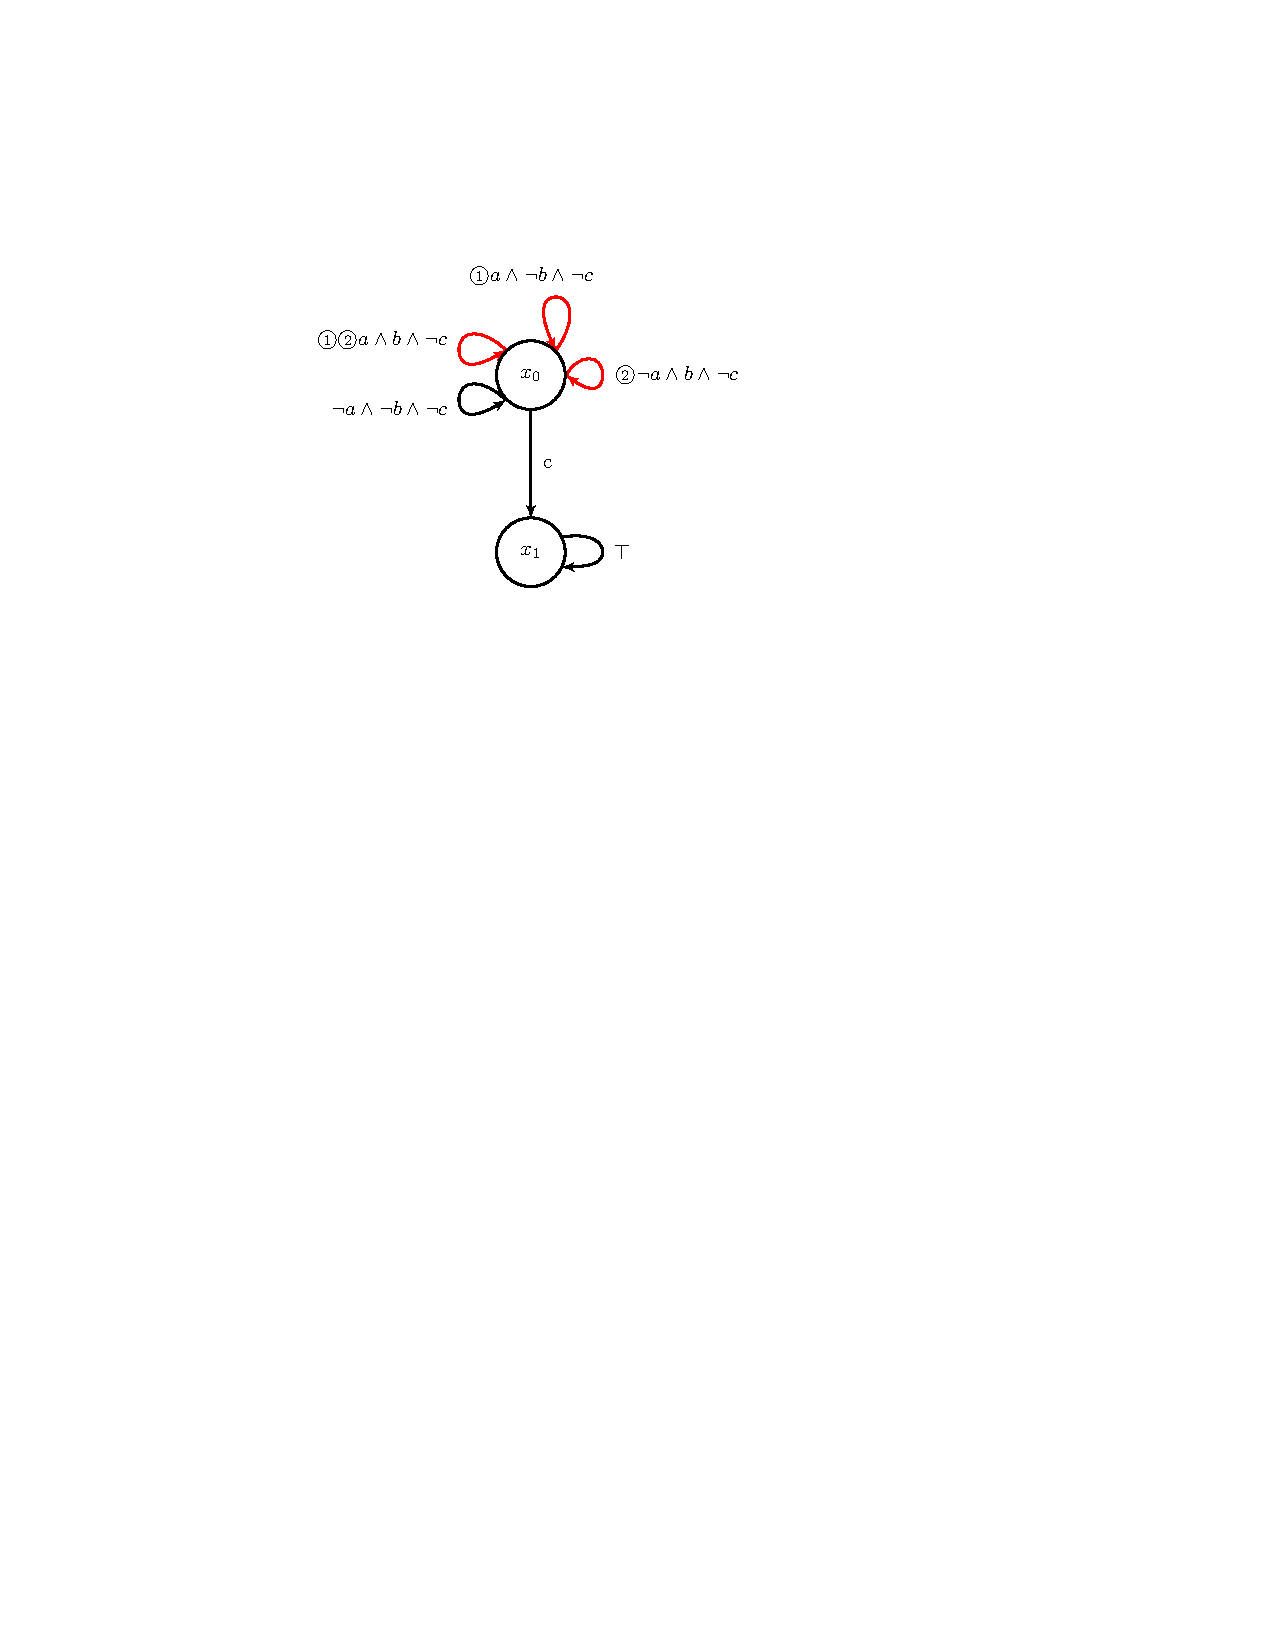
\includegraphics[bb=140 498 368 682,width=5cm]{automaton1.pdf}
   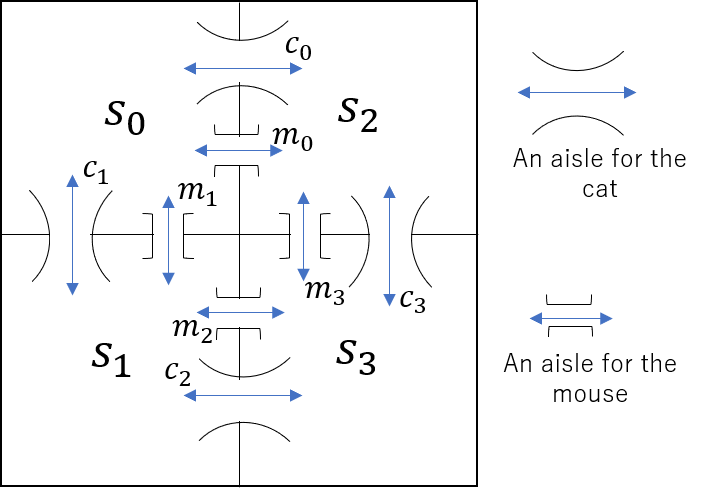
\includegraphics[width=7cm]{cat_mouse.png}
   \caption{The maze of the cat and the mouse. the initial state of the cat and the mouse is $s_0$ and $s_2$, respectively. the food for them is in the room 1 ($s_1$).}
   \label{cat_mouse}
\end{figure}

\begin{figure}[htbp]
   \centering
   \vspace{2mm}
%   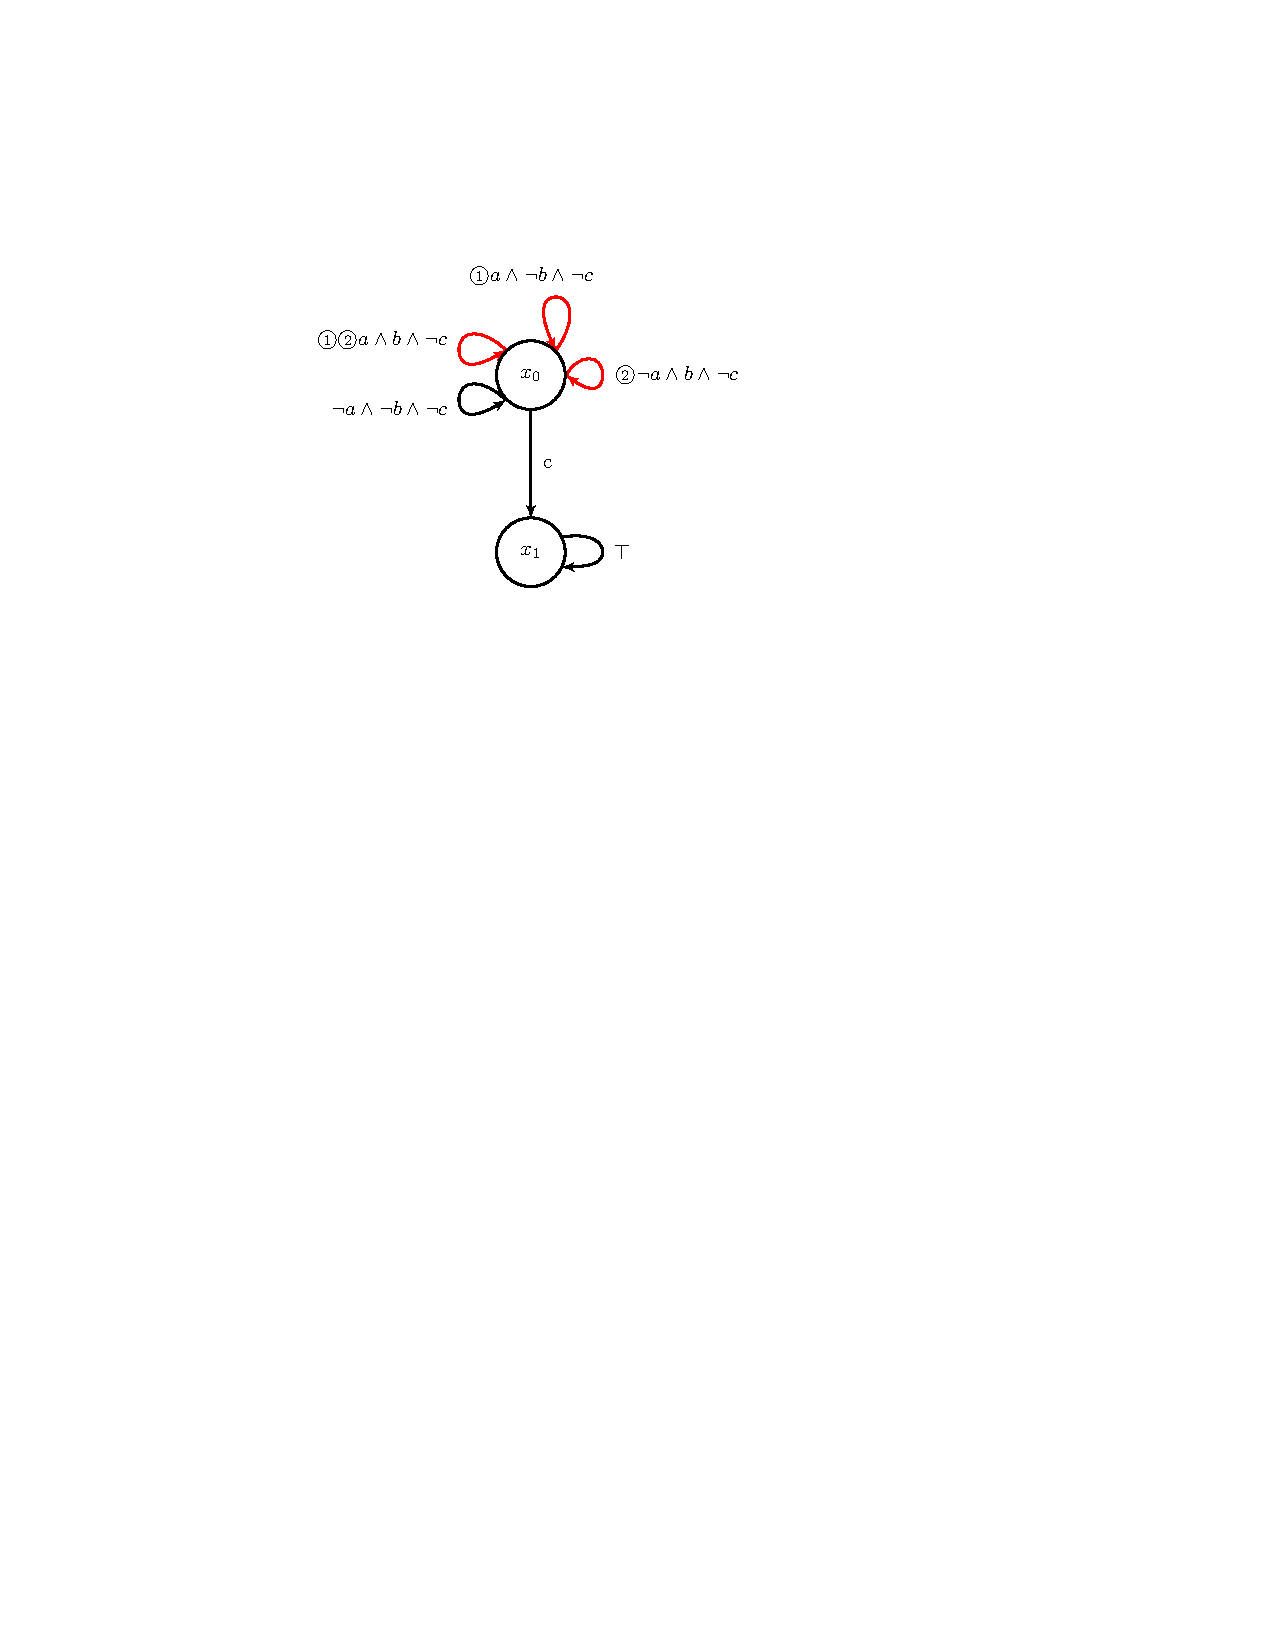
\includegraphics[bb=140 498 368 682,width=5cm]{automaton1.pdf}
   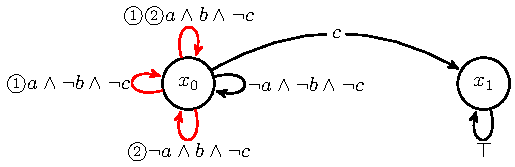
\includegraphics[bb=0 0 247 80,scale=0.85]{ldgba_original.pdf}
   \caption{The tLDBA recognizing the LTL formula $\text{{\bf GF}}a \wedge \text{{\bf GF}}b \wedge \text{{\bf G}}\neg c$, where the initial state is $x_0$. Red arcs are accepting transitions that are numbered in accordance with the accepting sets they belong to, e.g., \textcircled{\scriptsize 1}$a \land \neg b \land \neg c$ means the transition labeled by it belongs to the accepting set $F_1$.}
   \label{tldba}
\end{figure}

\begin{figure}[htbp]
   \centering
   \vspace{2mm}
%   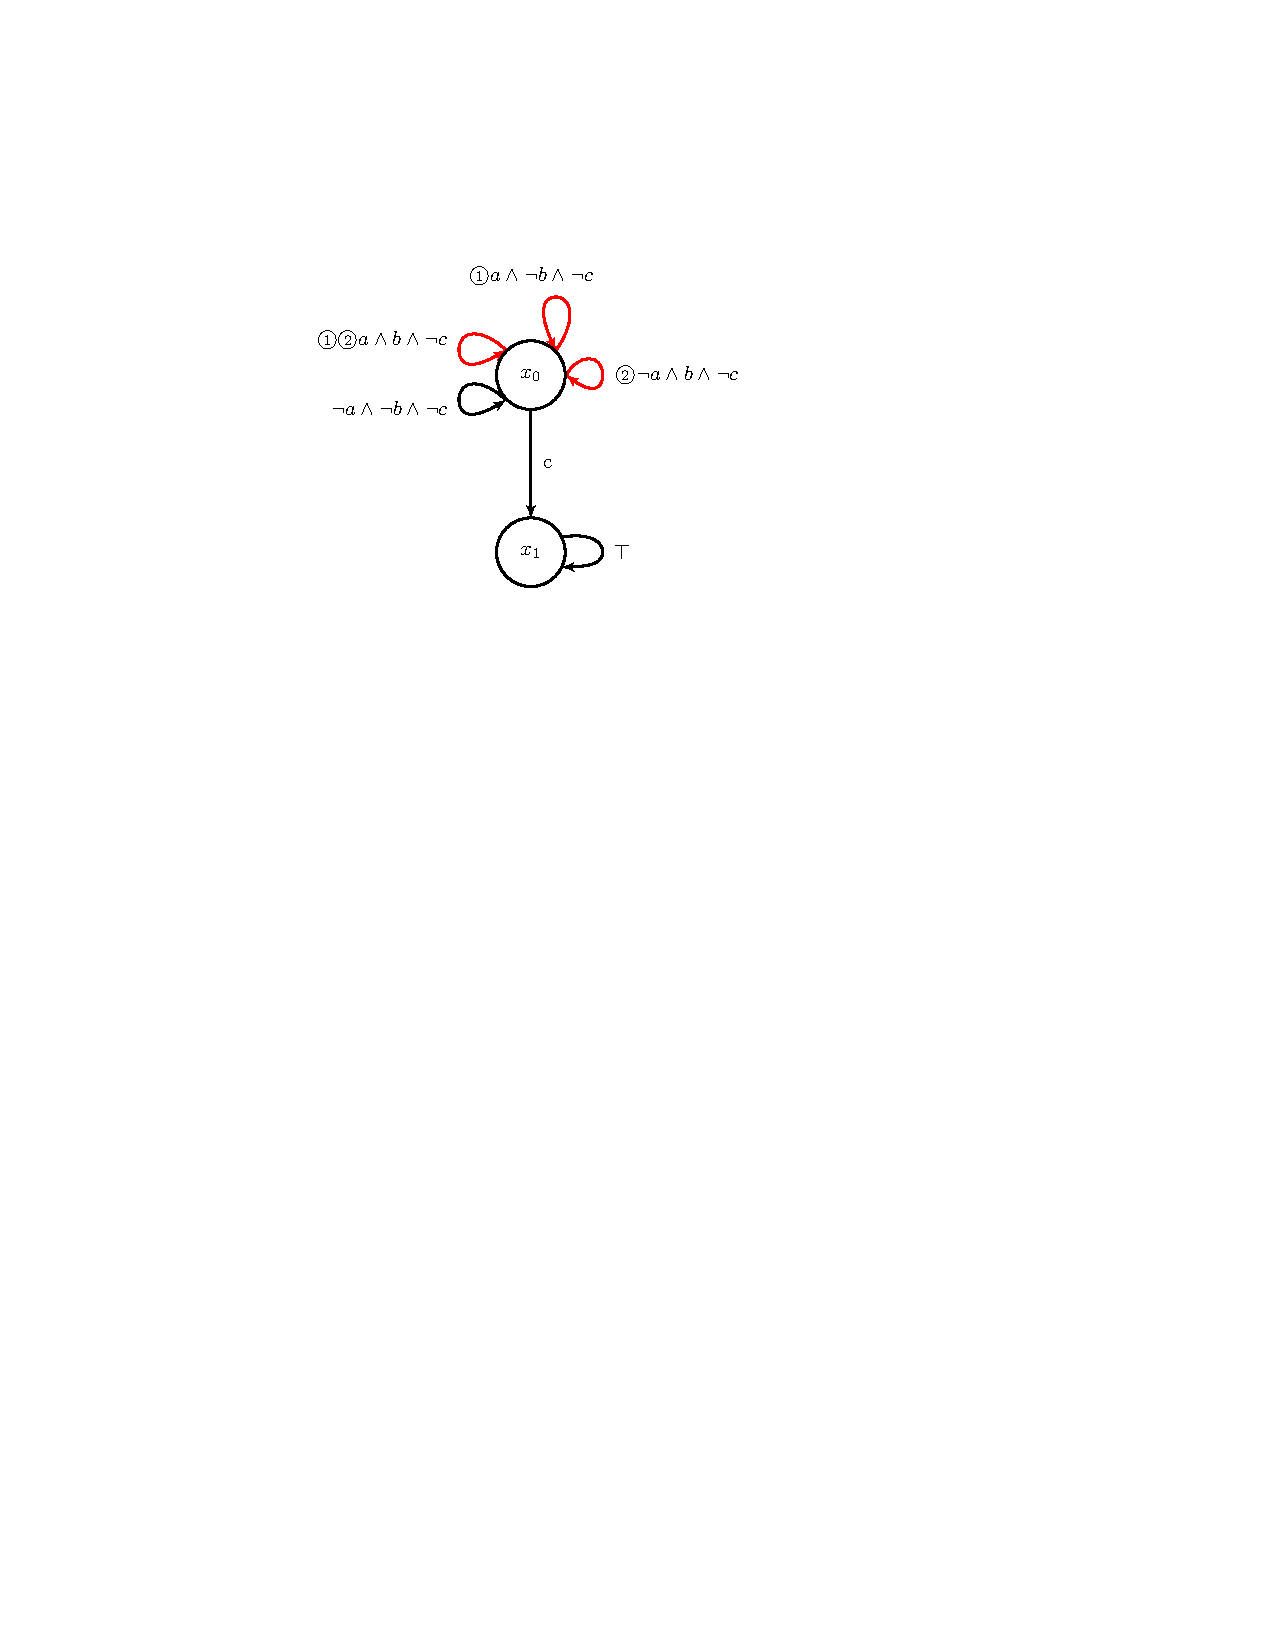
\includegraphics[bb=140 498 368 682,width=5cm]{automaton1.pdf}
   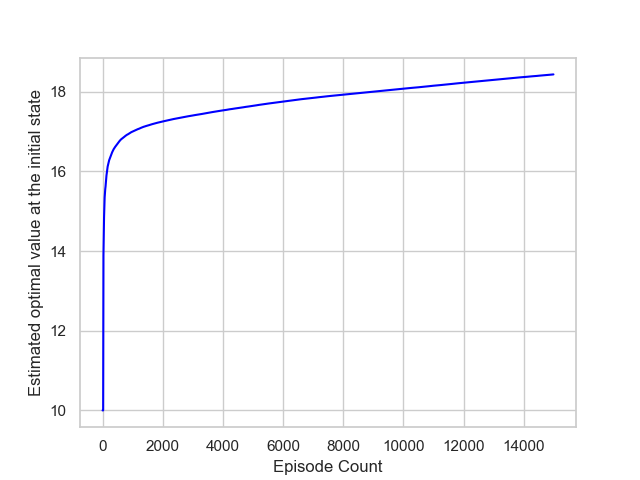
\includegraphics[width = 8cm]{max_Q_value_TD.png}
   \caption{The estimated optimal state value function at the initial state $V(s^{\otimes}_{init})$ with $r_{n1} = -0.1$ when using Algorithm \ref{alg1}.}
   \label{result1}
\end{figure}

\begin{figure}[htbp]
   \centering
   \vspace{2mm}
%   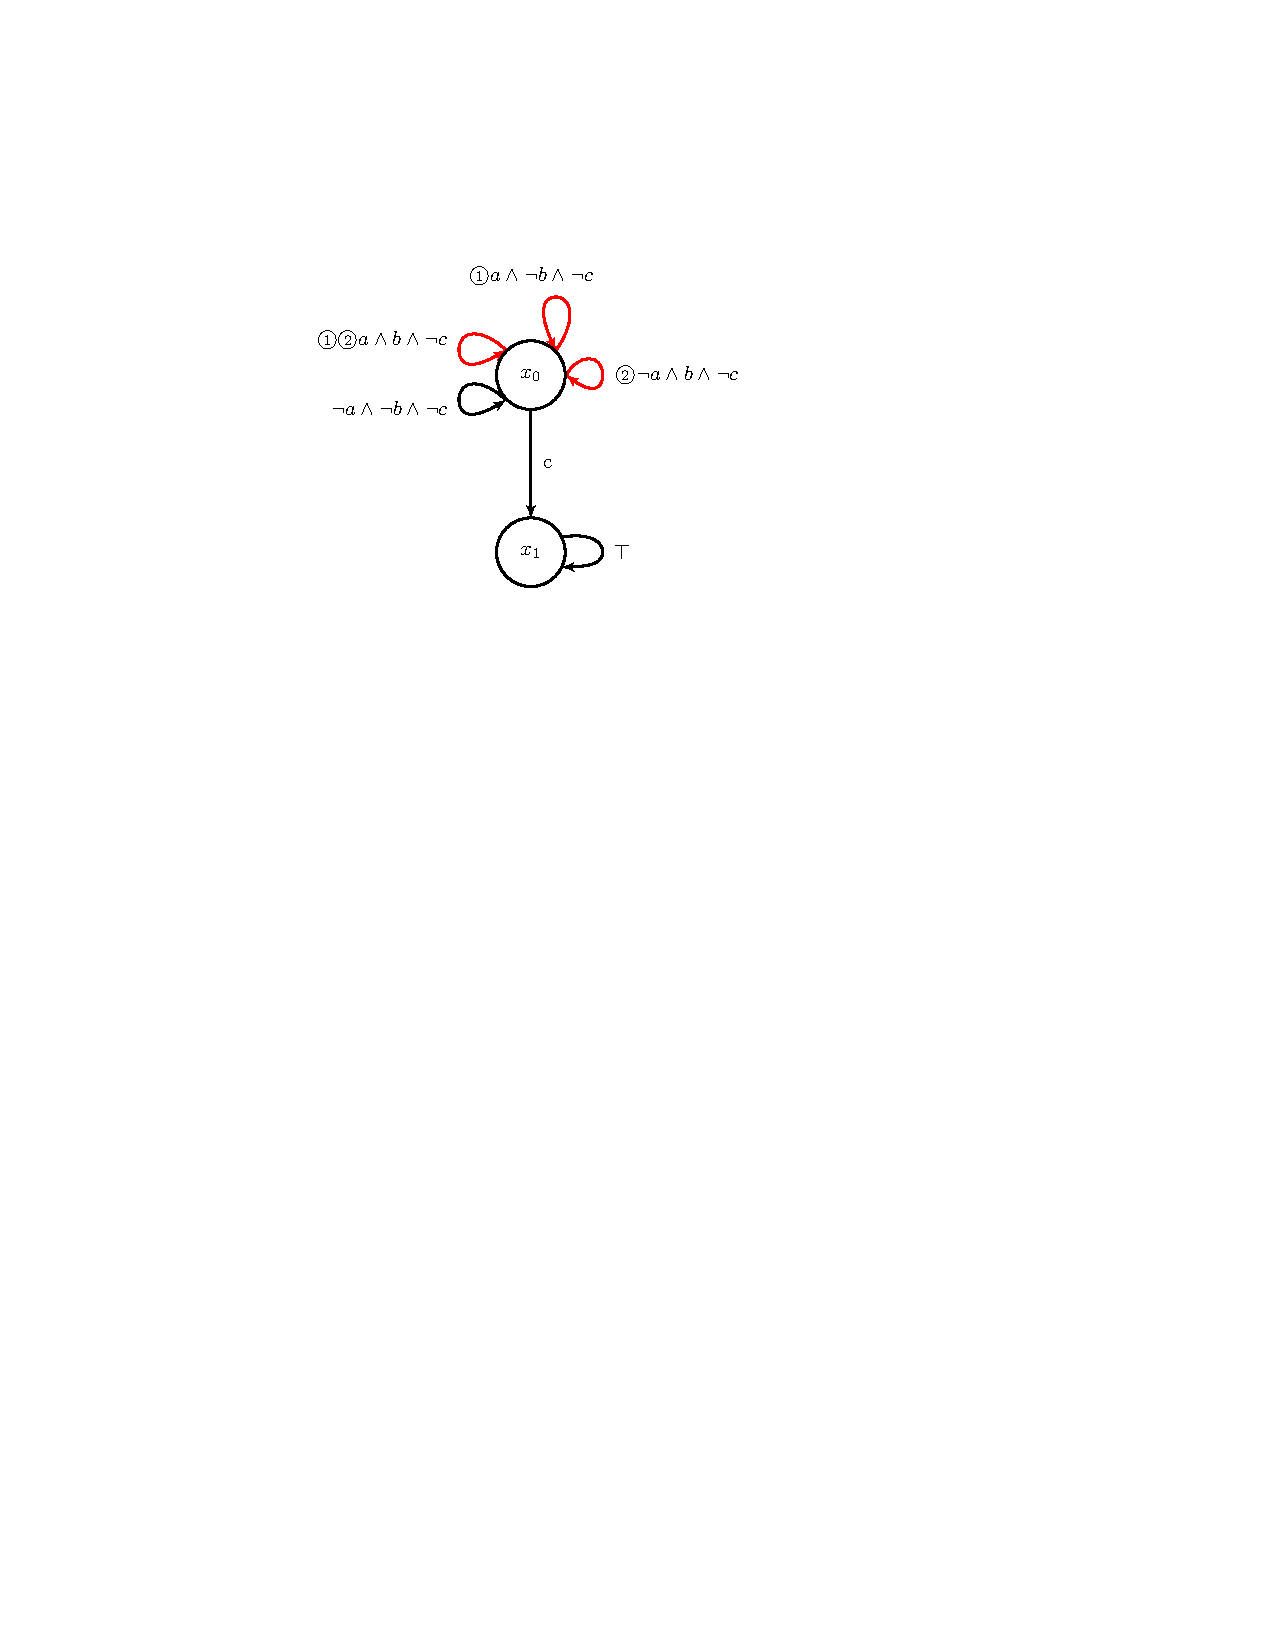
\includegraphics[bb=140 498 368 682,width=5cm]{automaton1.pdf}
   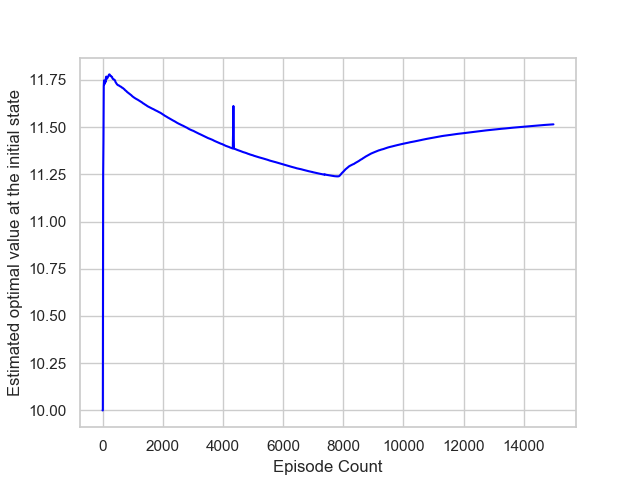
\includegraphics[width = 8cm]{learning_TD_v_15000_5000_rn2_05.png}
   \caption{The estimated optimal state value function at the initial state $V(s^{\otimes}_{init})$ with $r_{n1} = -0.5$ when using Algorithm \ref{alg1}.}
   \label{result2}
\end{figure}

\begin{figure}[htbp]
   \centering
   \vspace{2mm}
%   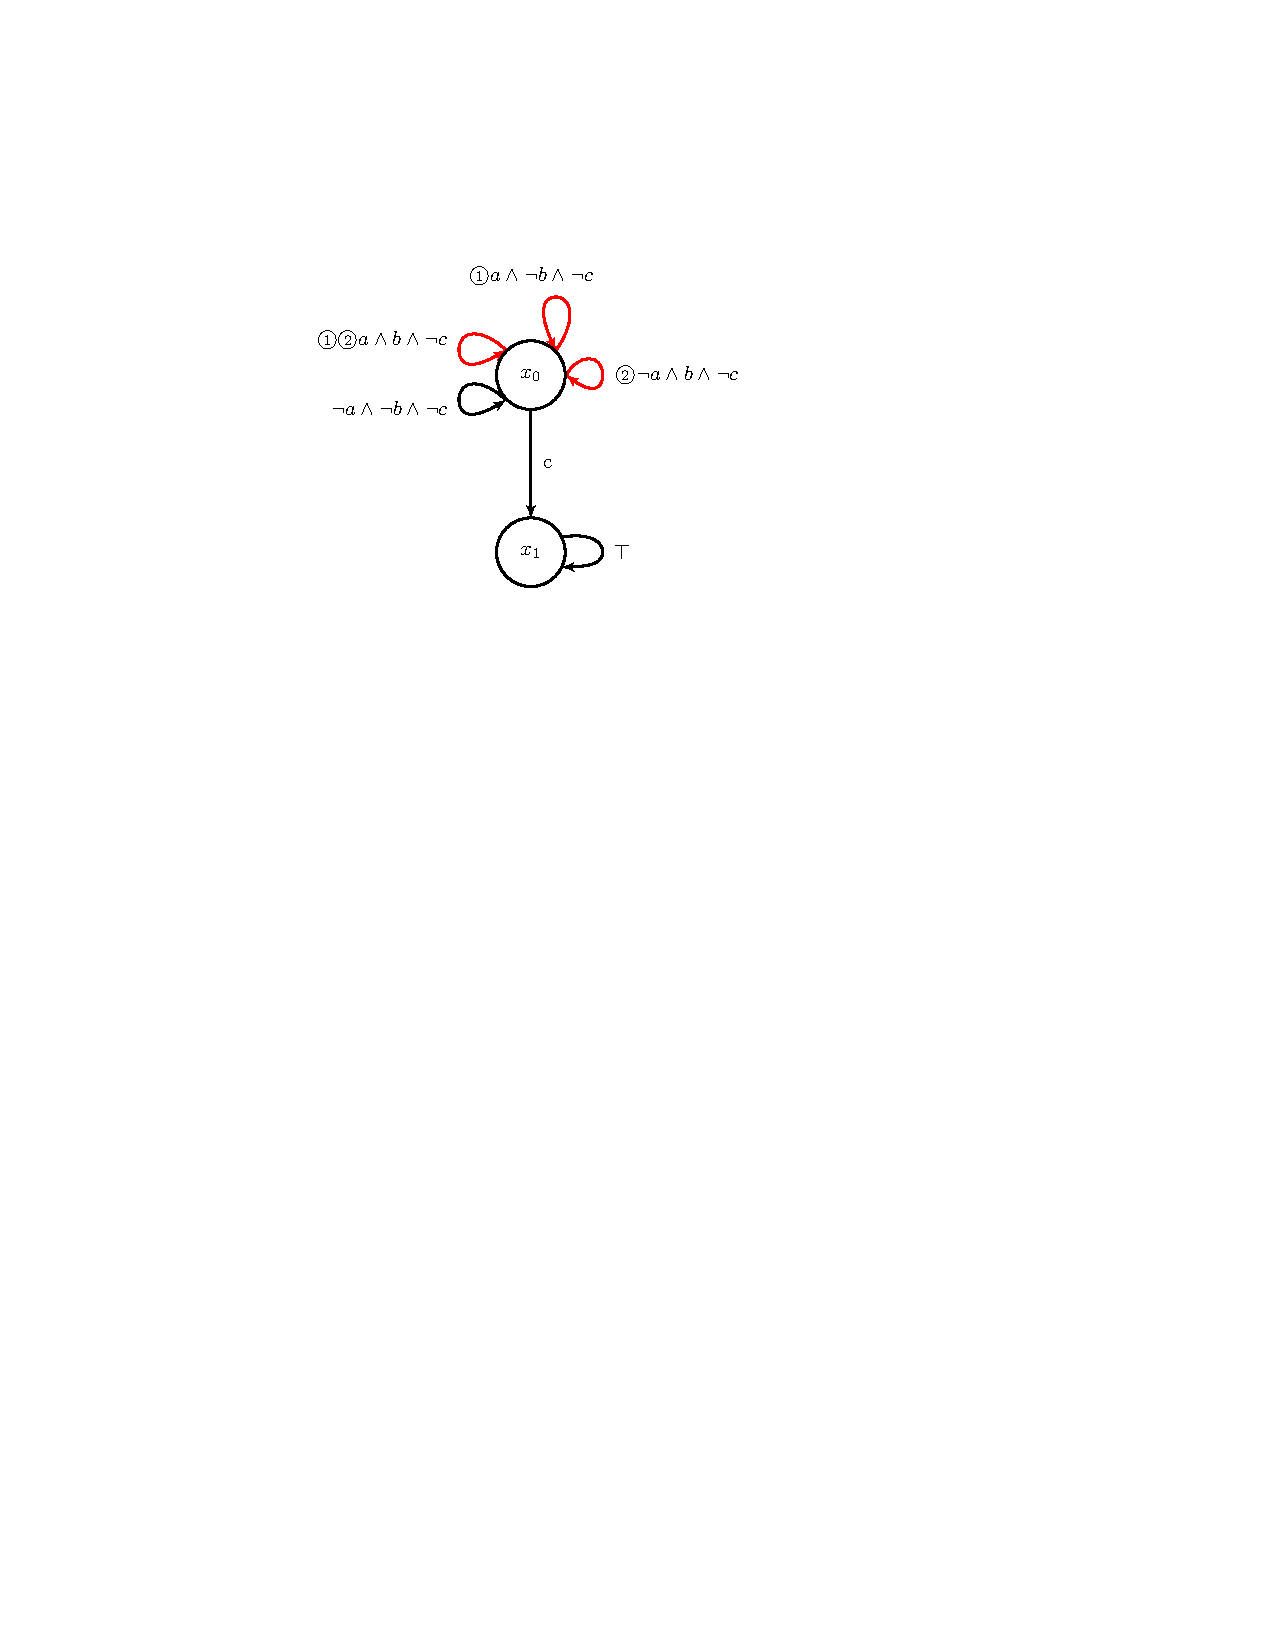
\includegraphics[bb=140 498 368 682,width=5cm]{automaton1.pdf}
   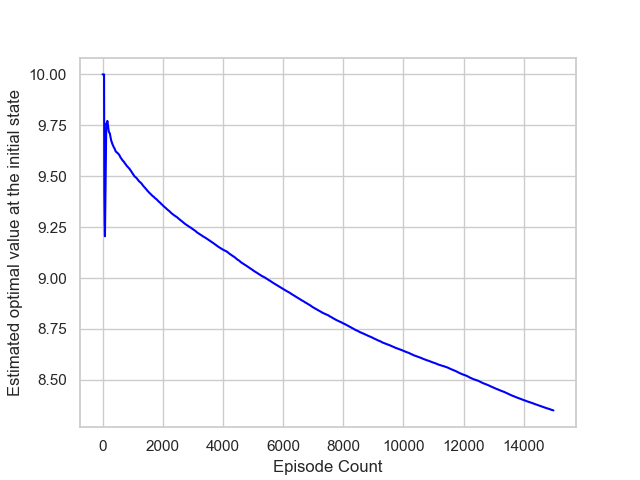
\includegraphics[width = 8cm]{max_Q_value_TD_rn2_1.png}
   \caption{The estimated optimal state value function at the initial state $V(s^{\otimes}_{init})$ with $r_{n1} = -1$ when using Algorithm \ref{alg1}.}
   \label{result3}
\end{figure}

\begin{figure}[htbp]
   \centering
   \vspace{2mm}
%   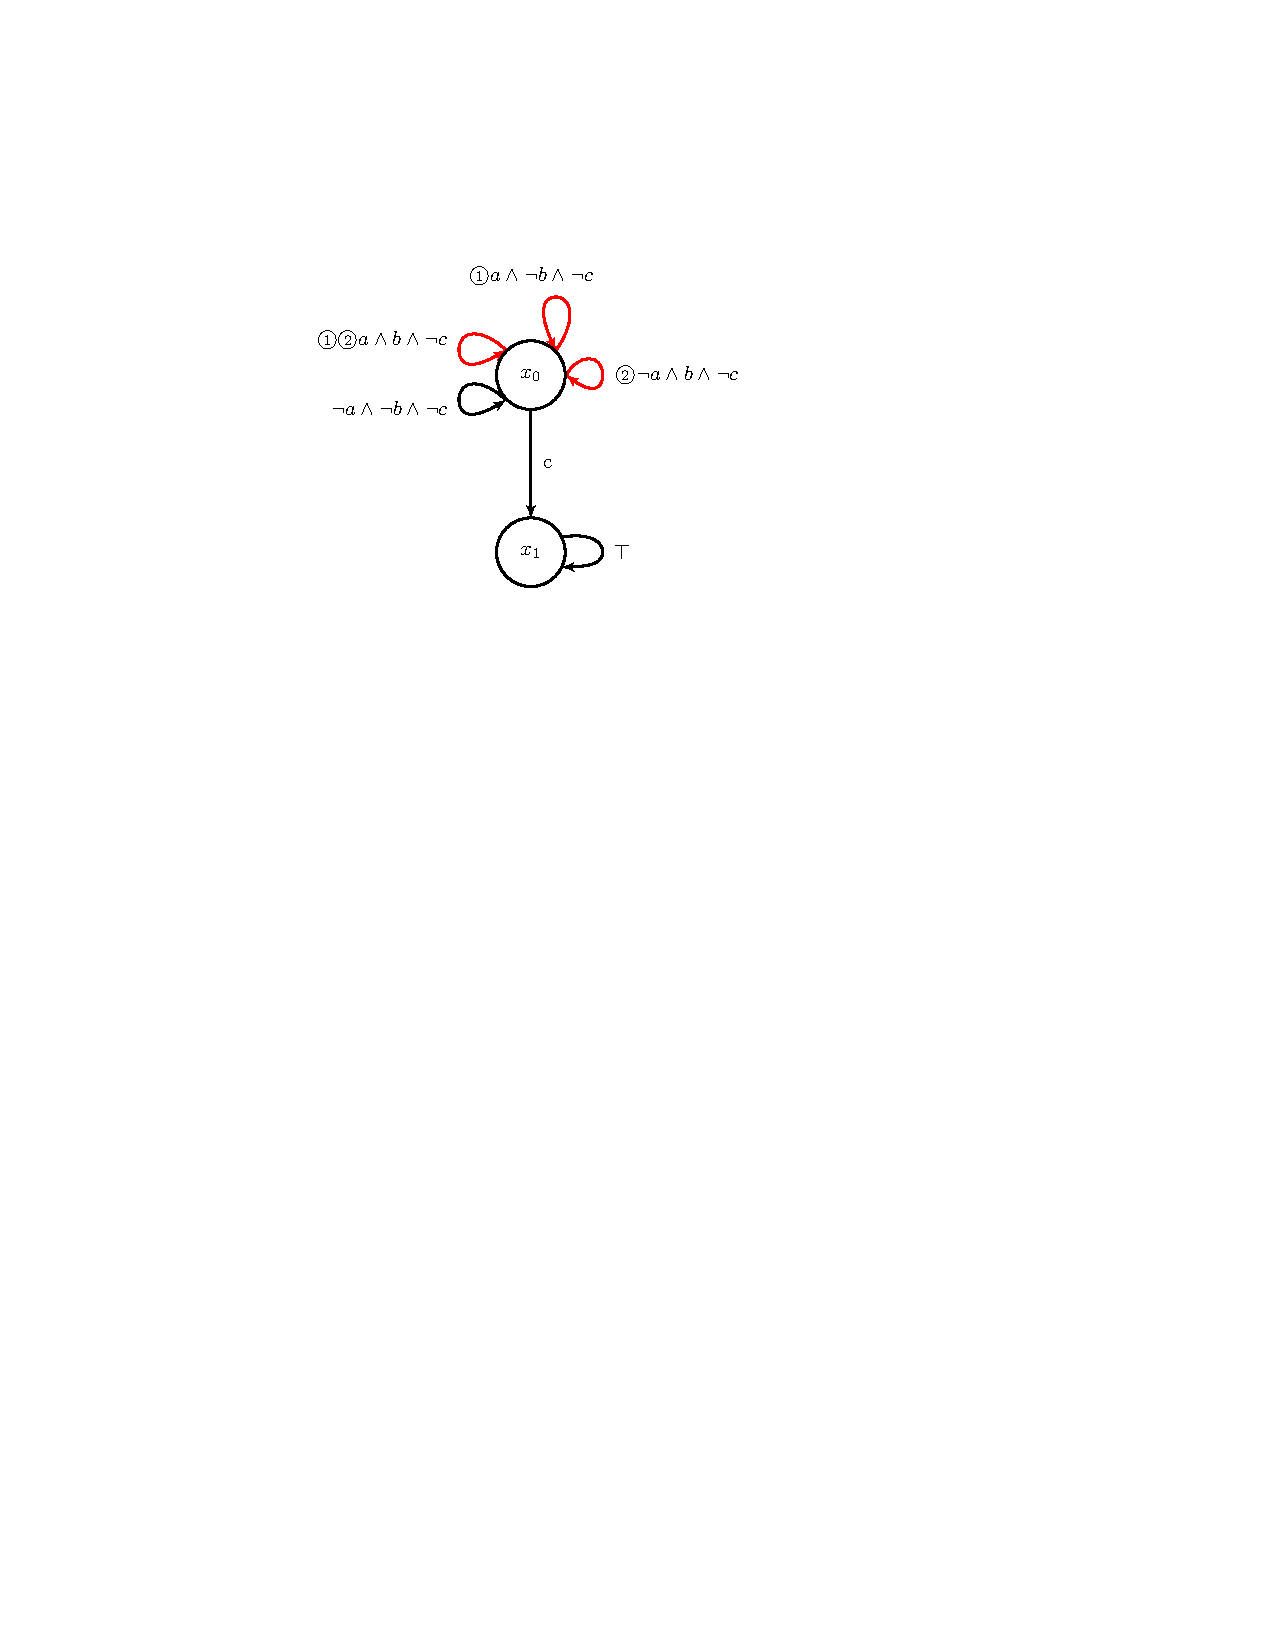
\includegraphics[bb=140 498 368 682,width=5cm]{automaton1.pdf}
   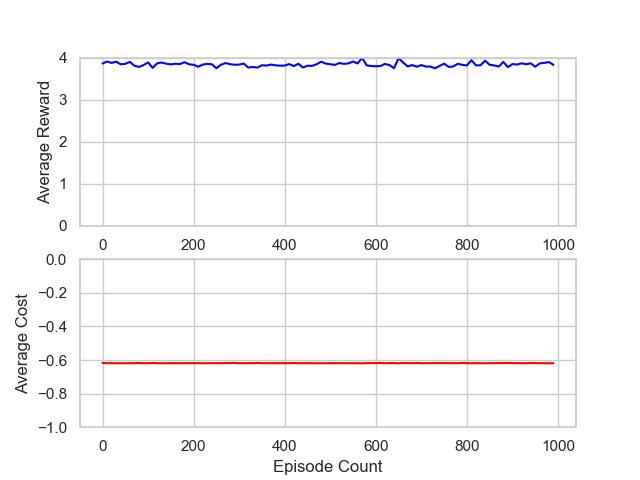
\includegraphics[width = 8cm]{simulate_TD_v_15000_5000.png}
   \caption{The average reward and average cost by the supervisor obtained from the learning with $r_{n1} = -0.1$.}
   \label{sim1}
\end{figure}

\begin{figure}[htbp]
   \centering
   \vspace{2mm}
%   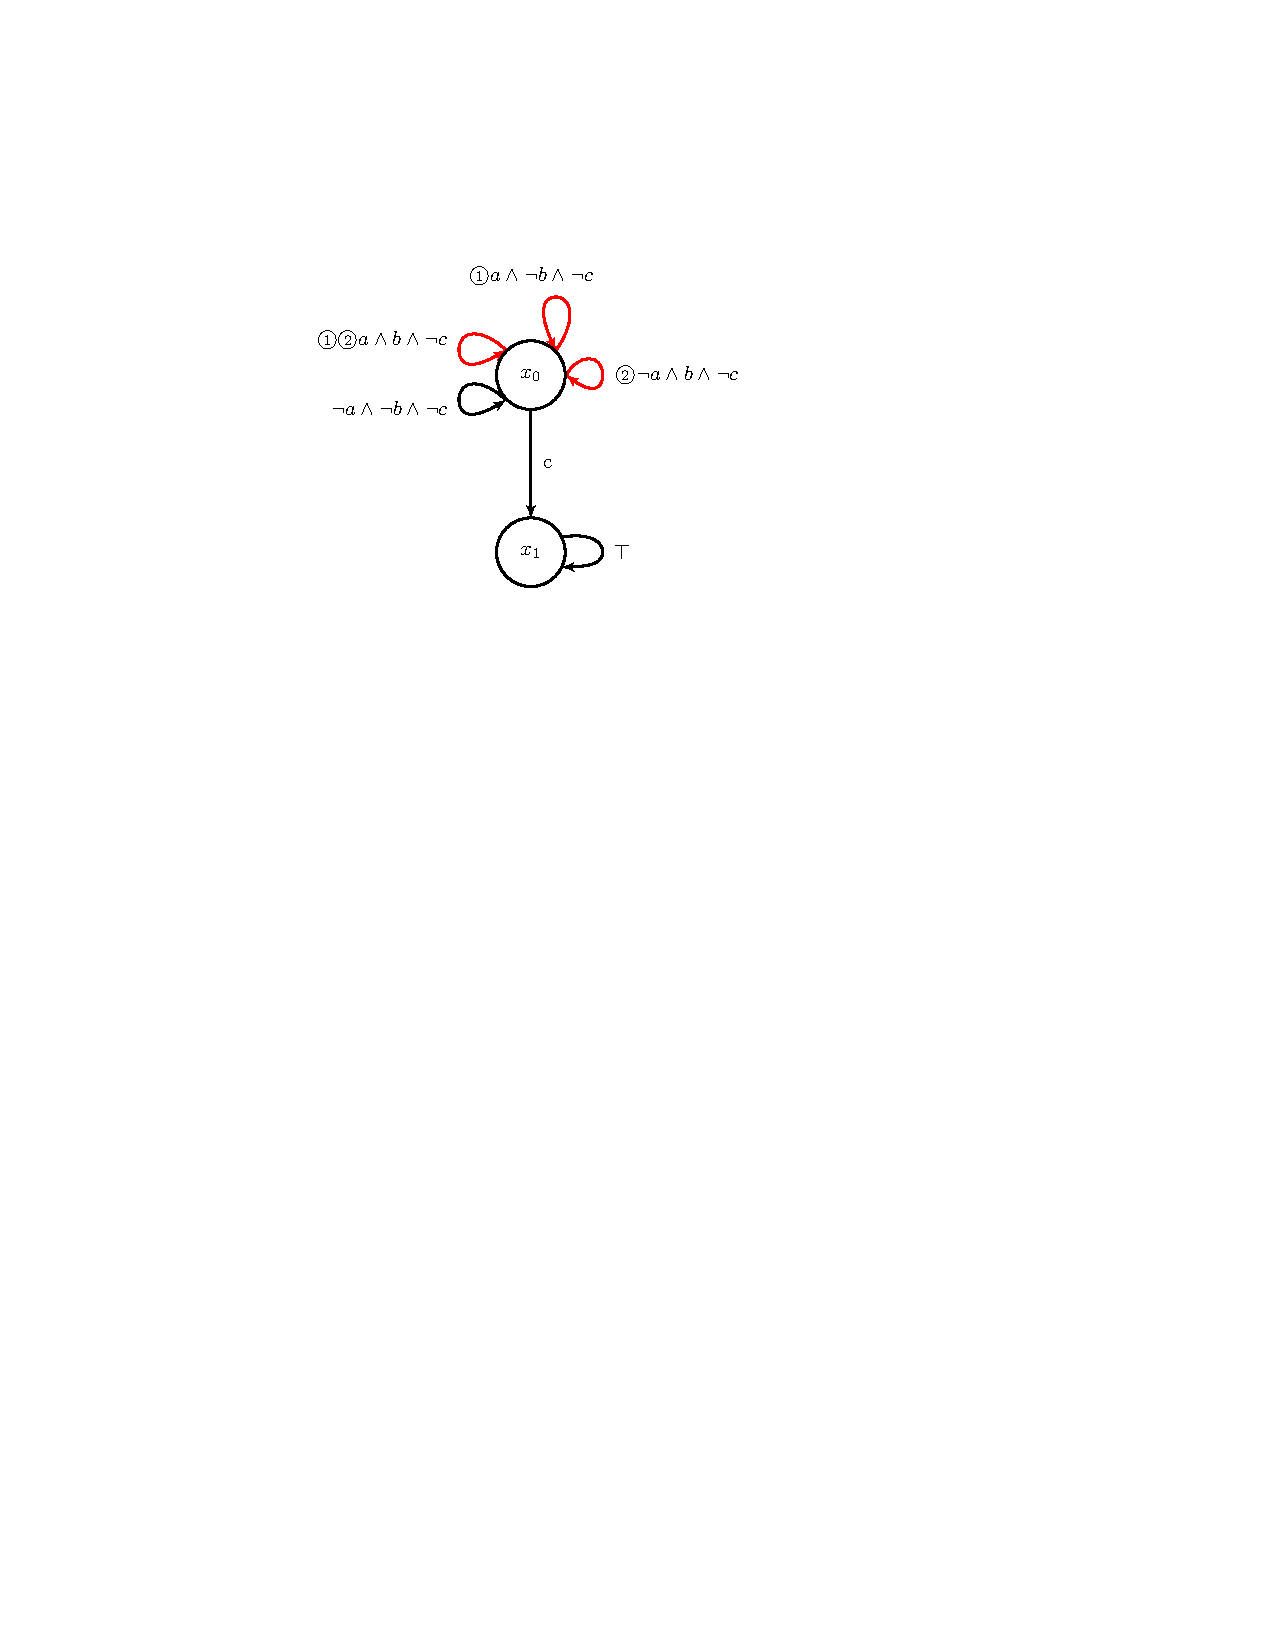
\includegraphics[bb=140 498 368 682,width=5cm]{automaton1.pdf}
   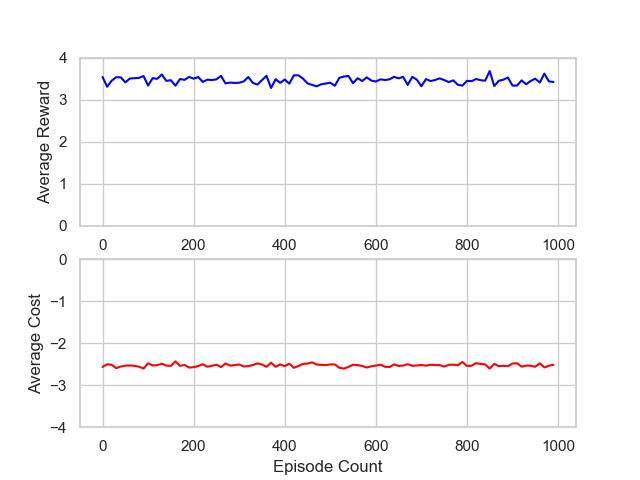
\includegraphics[width = 8cm]{simulate_TD_v_15000_5000_rn2_05.png}
   \caption{The average reward and average cost by the supervisor obtained from the learning with $r_{n1} = -0.5$.}
   \label{sim2}
\end{figure}

\begin{figure}[htbp]
   \centering
   \vspace{2mm}
%   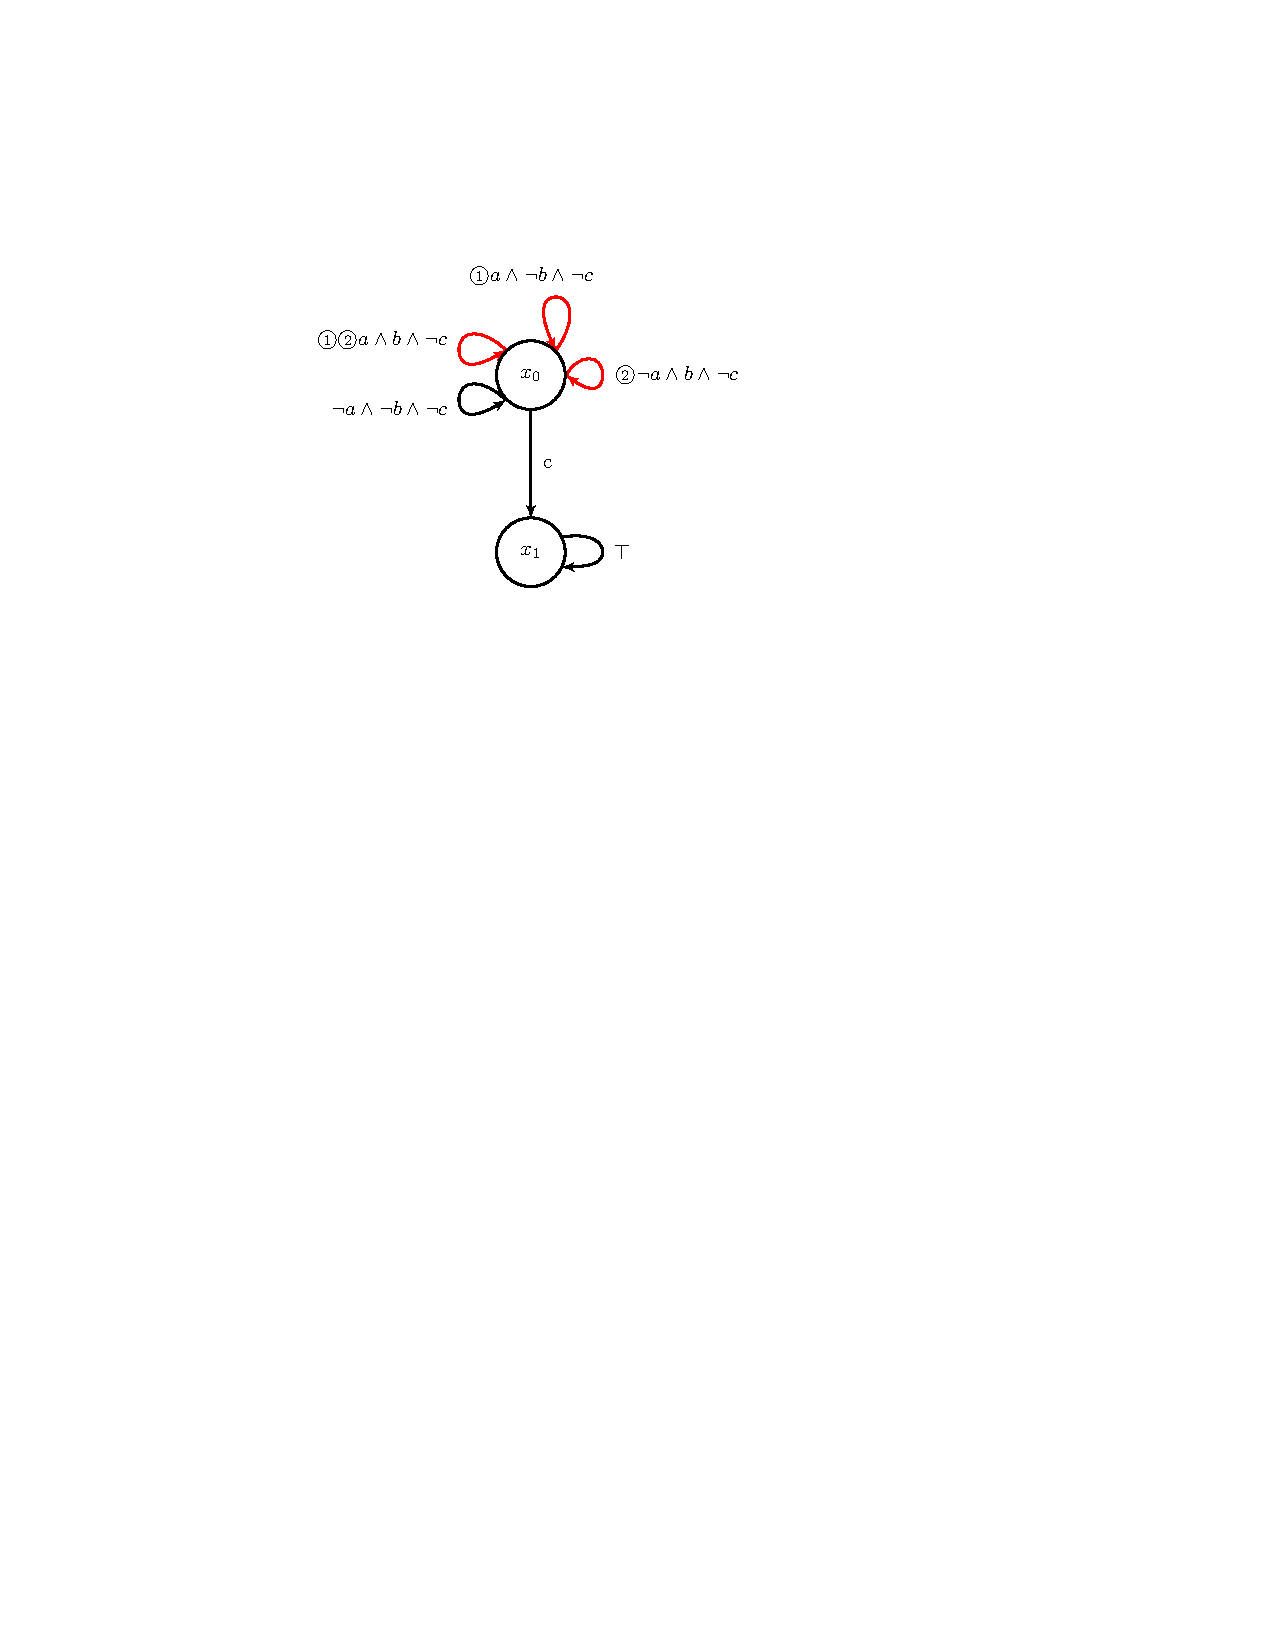
\includegraphics[bb=140 498 368 682,width=5cm]{automaton1.pdf}
   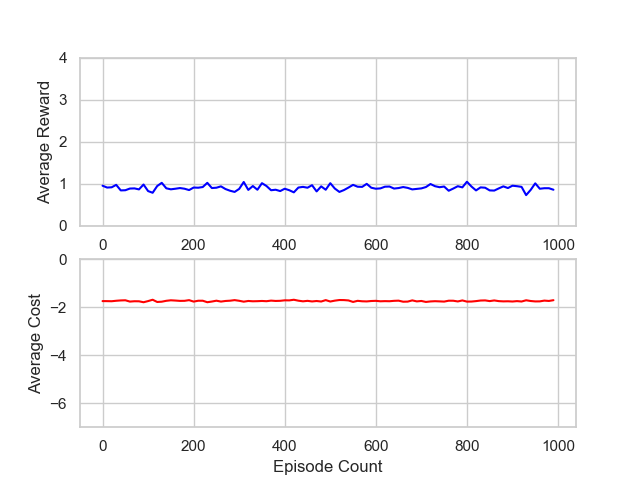
\includegraphics[width = 8cm]{simulate_TD_v_10000_5000_rn2_1.png}
   \caption{The average reward and average cost by the supervisor obtained from the learning with $r_{n1} = -1$.}
   \label{sim3}
\end{figure}

\begin{comment}
\begin{align}
   L((s, a, s^{\prime})) =
    \left\{
    \begin{aligned}
      & \{ a \} &  & \text{if }s_c^{\prime} = s_1, \nonumber \\
      & \{ b \} &  & \text{if }s_m^{\prime} = s_1, \nonumber \\
      & \{ c \} &  & \text{if }s_c^{\prime} = s_2, \nonumber \\
      & \{ d \} &  & \text{if }s_m^{\prime} = s_4, \nonumber \\
      & \{ e \} &  & \text{if }s_c^{\prime} = s_m^{\prime}, \nonumber \\
      & \emptyset &  & \text{otherwise},
    \end{aligned}
    \right.
\end{align}
where $s_c^{\prime}$ and $s_m^{\prime}$ is the next room where the cat and mouse is, respectively, i.e., $s^{\prime} = (s_c^{\prime},s_m^{\prime})$.

In the example, we want the supervisor to learn to give control patterns satisfying that the cat and the mouse take the food in room 1 ($s_1$) back to each room ($s_2$ and $s_4$) avoiding they come across. This is formally specified by the following LTL formula.
\begin{align*}
  \varphi = \text{{\bf GF}}a \wedge \text{{\bf GF}}b \wedge \text{{\bf GF}}c \wedge \text{{\bf GF}}d \wedge \text{{\bf G}}\neg e.
\end{align*}
The tLDBA $B_{\varphi} = (X, x_{init},\Sigma,\delta,\mathcal{F})$ corresponding to $\varphi$ is shown in Fig.\ \ref{tLDBA}.
\end{comment}


\end{document}
